\documentclass[a4]{scrartcl}

% \usepackage[ngerman]{babel}
\usepackage[utf8]{inputenc}
\usepackage{mathtools}
\usepackage{amsmath}
\usepackage{amssymb}
\usepackage{geometry}
\usepackage{scrlayer-scrpage}
\pagestyle{scrheadings}
\usepackage{tablefootnote}
\usepackage[dvipsnames]{xcolor}
% \clearscrheadfoot

\setlength{\parindent}{0em}

\setlength{\parskip}{1.3ex}

\usepackage[onehalfspacing]{setspace}


\clubpenalty = 10000
\widowpenalty = 10000
\displaywidowpenalty = 10000

\usepackage{hyperref}
\hypersetup{
	colorlinks=true,
	linkcolor=black,
	filecolor=black,      
	urlcolor=MidnightBlue,
	citecolor=black
}


\geometry{
	paper=a4paper, % Change to letterpaper for US letter
	top=3cm, % Top margin
	bottom=3cm, % Bottom margin
	left=2cm, % Left margin
	right=3cm, % Right margin
	%showframe, % Uncomment to show how the type block is set on the page
}

\usepackage[backend=biber, maxbibnames=99]{biblatex}
\addbibresource{references.bib}



\usepackage[framemethod=TikZ]{mdframed}

% Style %
\mdfdefinestyle{enviStyle}{
	innertopmargin = 10pt,
	linewidth      = 1pt,
	frametitlerule = true,
	roundcorner    = 2pt%
}


\usepackage{sectsty}
\sectionfont{\color{MidnightBlue}}
\subsectionfont{\color{MidnightBlue}}



\newenvironment{CountingDefinition}[2][]{%
	\ifstrempty{#1}%
	{\mdfsetup{%
			frametitle={{\strut ~}}}
	}%
	{\mdfsetup{%
			frametitle={{\strut ~#1}}}%
	}%
	\mdfsetup{
		nobreak                   = true,
		linecolor                 = MidnightBlue,
		frametitlebackgroundcolor = MidnightBlue!50,
		style                     = enviStyle
	}
	\begin{mdframed}[]\relax%
		\label{#2}}{\end{mdframed}}



\renewcommand{\labelitemi}{$\textcolor{MidnightBlue}{\bullet}$}
\renewcommand{\labelitemii}{$\textcolor{MidnightBlue}{\cdot}$}
\renewcommand{\labelitemiii}{$\textcolor{MidnightBlue}{\diamond}$}
\renewcommand{\labelitemiv}{$\textcolor{MidnightBlue}{\ast}$}





%\ohead{\\
%	Pina Kolling\\
%	piko0011}

\begin{document}
	
	\begin{titlepage}
		\centering
		{\scshape\LARGE Umeå University \par}
		\vspace{1cm}
		{\scshape\Large Managing the Digital Enterprise \par }
		\vspace{1.5cm}
		{\huge\bfseries   {\color{MidnightBlue}Individual Assignment 4} \par}
		\vspace{2cm}
		{\Large\itshape Pina Kolling\par}
		\vfill
		supervised by \par 
		\vspace{1cm}
		Dr. Daniel \textsc{Skog} \par 
		and \par 
		M. Sc. Ramy \textsc{Shenouda} 
		
		\vfill
		
		% Bottom of the page
		{\large \today\par}
	\end{titlepage}
	
	\setcounter{page}{1}
	
	\begin{doublespace}
		\tableofcontents
	\end{doublespace}

	
	\newpage

%The concept of digital transformation is understood differently by different people in both research and practice. Considering the amount of resources that are being invested in strategic digital transformation initiatives, it is of vital importance that managers of digital enterprises have a clear view of what it entails. In particular, it is of high importance that managers understand the extent of change that is involved for the organization. Your task in this assignment is to provide a synthesis of research that a manager of a digital enterprise can use to understand when a change stemming from technology emergence and use should be considered a digital transformation and not. Based on your synthesis, your task is also to provide research-grounded advice on what a manager could expect and plan for when initiating digital transformation in the organization. Specifically, your task is to:












% 1. Value, select and summarize research concepts, perspectives and arguments from at least three of the papers below concerning when a process should be considered to be a digital transformation and not. 
%-------------------------------------------------------------------------------------------
	\section{Definitions of Digital Transformation} \label{sec:Sec1}







%-------------------------------------------------------------------------------------------	
	\subsection{\textit{Digital doesn't have to be disruptive}} \label{disruptive}
	
	The authors Nathan Furr and Andrew Shipilov described digital transformation in \textit{Digital doesn't have to be disruptive: the best results can come from adaptation rather than reinvention}~\cite{disruptive} as ``adapting an organization's strategy and structure to capture opportunities enabled by digital technology``~\cite[p. 96]{disruptive}.
	The main aspects of digital transformation are listed as automation, virtualization, more targeted product and service customization, more informed decision making and machine-driven recommendations. Those technologies can be applied at almost every company and in almost every step of their processes.~\cite{disruptive}
	
	It can be difficult for companies to create a plan on how to act and execute their digital transformation. But radical replacements are only sometimes necessary -- digital transformation means incremental steps to improve the processes. This includes getting more efficient and user-friendly using digital tools, finding the best way to reach the company's goals through digital tools or to overcome previous challenges.~\cite{disruptive}
	









%-------------------------------------------------------------------------------------------	
\subsection{\textit{Five myths about digital transformation}} \label{5myths}	
	
	Stephen J. Andriole stated in \textit{Five myths about digital transformation}~\cite{5myths} that the path to digital transformation can be risky, even if it might lead to efficiency, innovation and competitiveness.
	According to the author, companies will fail to implement digital transformation unless it is extremely well planned and executed. There were five myths about digital transformation collected and presented to raise awareness to the risks and dangers of digital transformation. The resulting guidelines from those five myths are summarized in the following.~\cite{5myths}
	\begin{enumerate}
		\item ``Not every company, process, or business model requires digital transformation``~\cite[p. 20]{5myths}
		\item Digital transformation does not necessarily use emerging or disruptive technologies.
		\item If the company is already thriving, the transformation will not have a meaningful impact.
		\item Disruptive transformation does usually not begin with the market leaders.
		\item The executives do not necessarily want to transform digitally.
	\end{enumerate}
	
	










%-------------------------------------------------------------------------------------------	
\subsection{\textit{IT-enabled business transformation}} \label{venkat}	

In \textit{IT-enabled business transformation: from automation to business scope redefinition}~\cite{venkat} by Nramanujam Venkatraman was stated that IT has a distinctive role in shaping the future's business operations while being a fundamental enabler in creating and maintaining competitiveness.
Five levels of digital transformation were introduced and it was suggested that companies should at first estimate the costs and efforts in comparison to the benefits and then move to higher levels of the transformation. Those levels are summarized in the following.~\cite{venkat}

\begin{description}
	\item[Level 1] Localized Exploitation: 
	
	Deployment of standard IT applications with minimal changes to the business processes.
	
	\item[Level 2] Internal Integration: 
	
	Deployment of IT applications in the entire business process.
	
	\item[Level 3] Business Process Redesign: 
	
	Renewing of processes to improve efficiency with IT applications.
	
	\item[Level 4] Business Network Redesign: 
	
	Execution of digital transformation not only within the organization but with partners or suppliers.
	
	\item[Level 5] Business Scope Redefinition: 
	
	Redefining the market and the company's goals and potentially outsource tasks to third party companies.
	
\end{description}


	
	
	
	
	
	
	
%-------------------------------------------------------------------------------------------	
\subsection{\textit{Understanding digital transformation}} \label{vial}	
	
Gregory Vial in \textit{Understanding digital transformation: A review and a research agenda}~\cite{vial} stated that digital transformation consists out of 8 building blocks: Digital technologies, disruption, strategic responses, value creation paths, structural changes, organizational barriers and positive and negative outcomes.
Those building blocks and their connection build a framework, that was visualized. This can be seen in Figure \ref{vial_framework}.~\cite{vial}

\begin{figure}[h!]
	\centering
	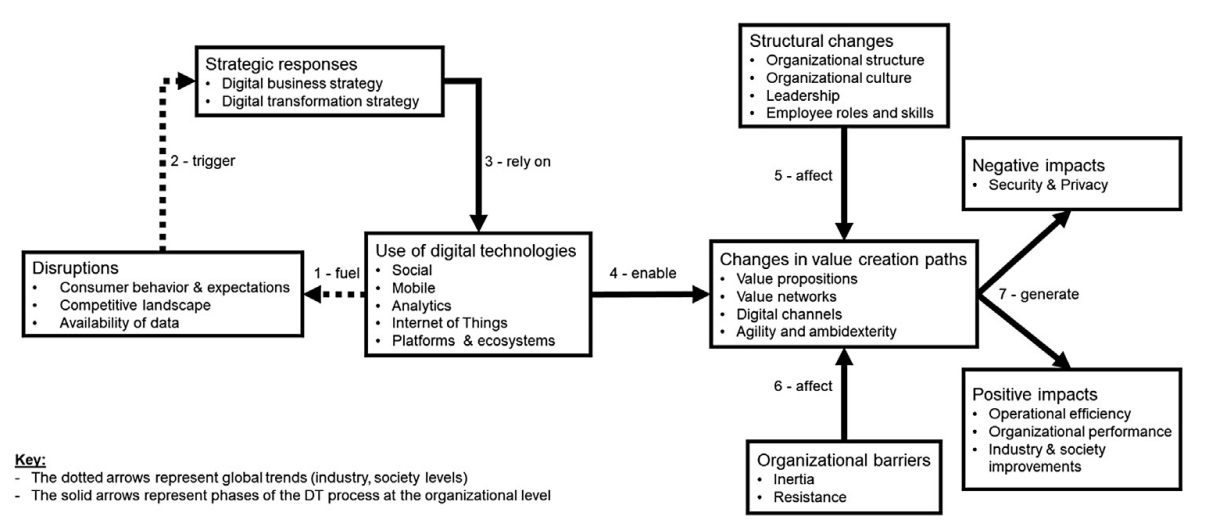
\includegraphics[width=1\textwidth]{images/vial.png}
	\caption{Digital transformation framework \cite{vial}}
	\label{vial_framework}
\end{figure}
	
TODO: describe this framework?

% table with different definitions of digital transformation









	





%-------------------------------------------------------------------------------------------	
\subsection{\textit{Digital Transformation versus IT-Enabled Transformation}} \label{DTOT}	

Lauri Wessel, Abayomi Baiyere, Roxana Ologeanu-Taddei, Jonghyuk Cha and Tina Blegind-Jensen in \textit{Unpacking the difference between digital transformation and IT-enabled organizational transformation}~\cite{DTOT} focus on the difference between digital transformation and IT-enabled transformation.
It is stated that digital transformation can lead to a new organizational identity while IT-enabled organizational transformation is the enhancement of an existing organizational identity.~\cite{DTOT}
	














% 2. Analyze and synthesize the concepts, perspectives and arguments to individually argue for 3-4 key characteristics that can be used to determine whether a process should be considered to be a digital transformation and not. 
%-------------------------------------------------------------------------------------------
\section{Section 2} \label{sec:Sec2}

\begin{CountingDefinition}[Definitions]{def:defdef}
	
		
		Text

	
	
\end{CountingDefinition}











% 3. Use the 3-4 key characteristics to explain what scope and scale of change a manager should expect and plan for when initiating a digital transformation initiative and the most important things a manager needs to think about to manage it successfully
%-------------------------------------------------------------------------------------------
\section{Section 3} \label{sec:Sec3}

\begin{CountingDefinition}[Definitions]{def:defdef}
	

		
		Text

	
\end{CountingDefinition}













%-------------------------------------------------------------------------------------------
	
	\newpage
	\addcontentsline{toc}{section}{References}
	\begin{spacing}{0.9}
		\printbibliography
	\end{spacing}


	
	
	
	
	
	
\end{document}